\addcontentsline{toc}{chapter}{Appendices}

% The \appendix command resets the chapter counter, and changes the chapter numbering scheme to capital letters.
%\chapter{Appendices}
%%%%%%%%%%%%%%%%%%%%%%%%%%%%%%%%%%%%%%%%%%%%%%%%%%%%%%%%%%%%%%%
%% APPENDIX 1
\appendix
\chapter{Coil sensitivity profiles by number of channels}
\label{appendixlabel1}

\begin{figure}[H]
    \centering
    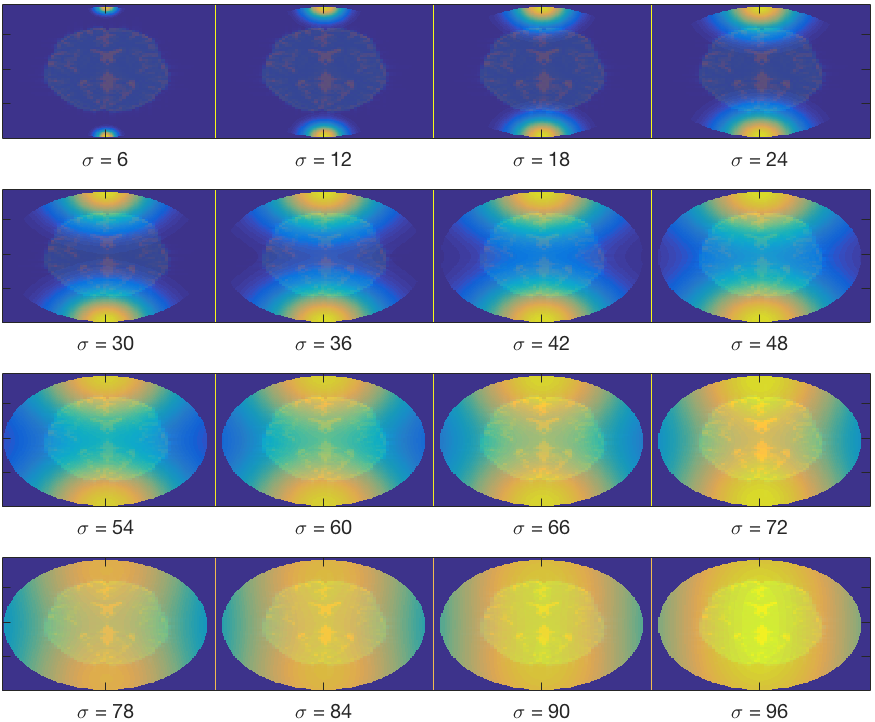
\includegraphics[width=.8\textwidth,keepaspectratio]{2coilsdifsigmas}
    \caption{Coil sensitivity maps of the 2-channel arrangement}
\end{figure}

\begin{figure}[H]
    \centering
    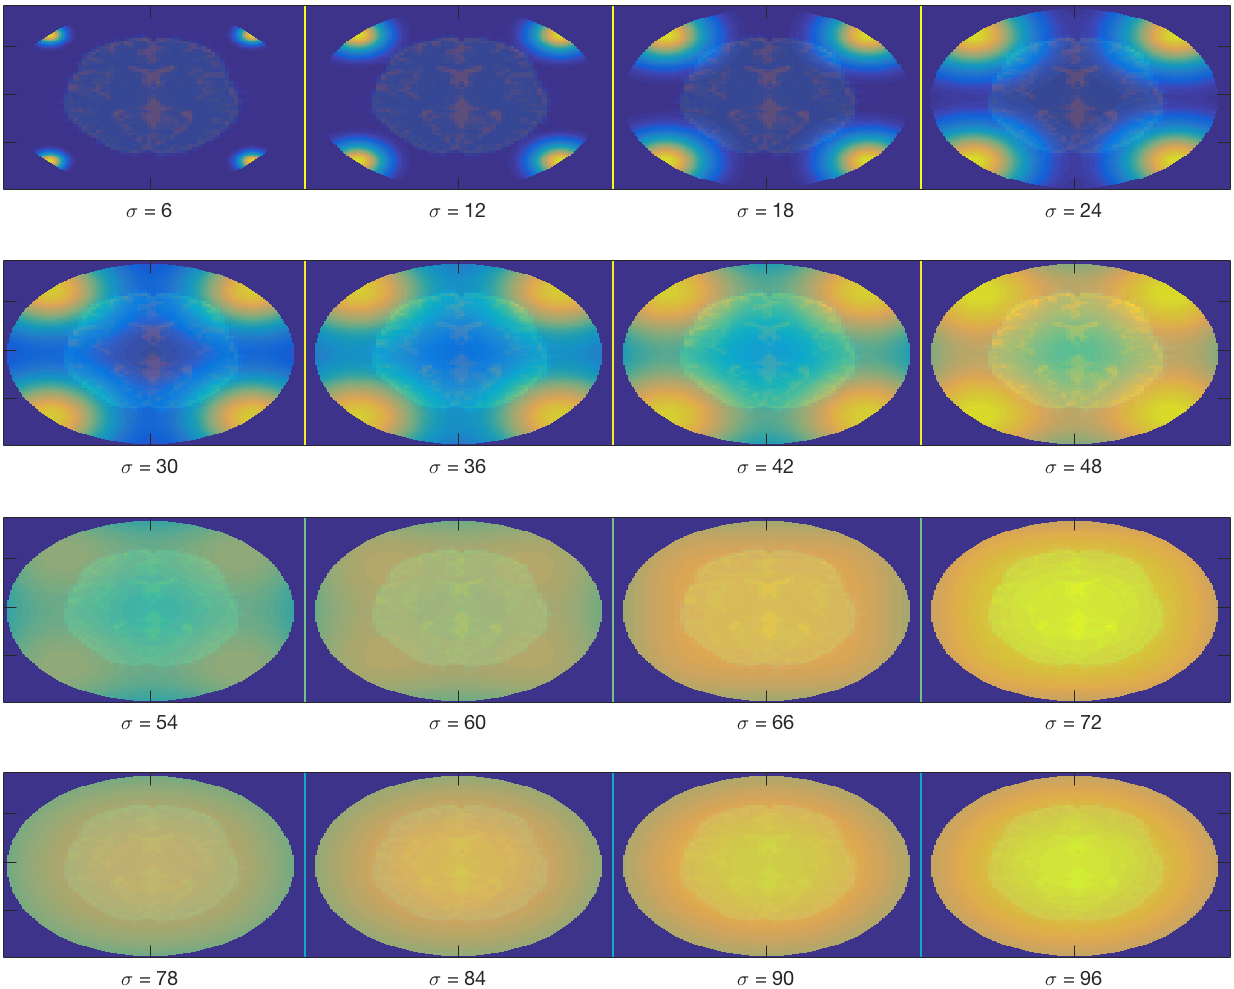
\includegraphics[width=.8\textwidth,keepaspectratio]{4coilsdifsigmas}
    \caption{Coil sensitivity maps of the 4-channel arrangement}
\end{figure}

\begin{figure}[H]
    \centering
    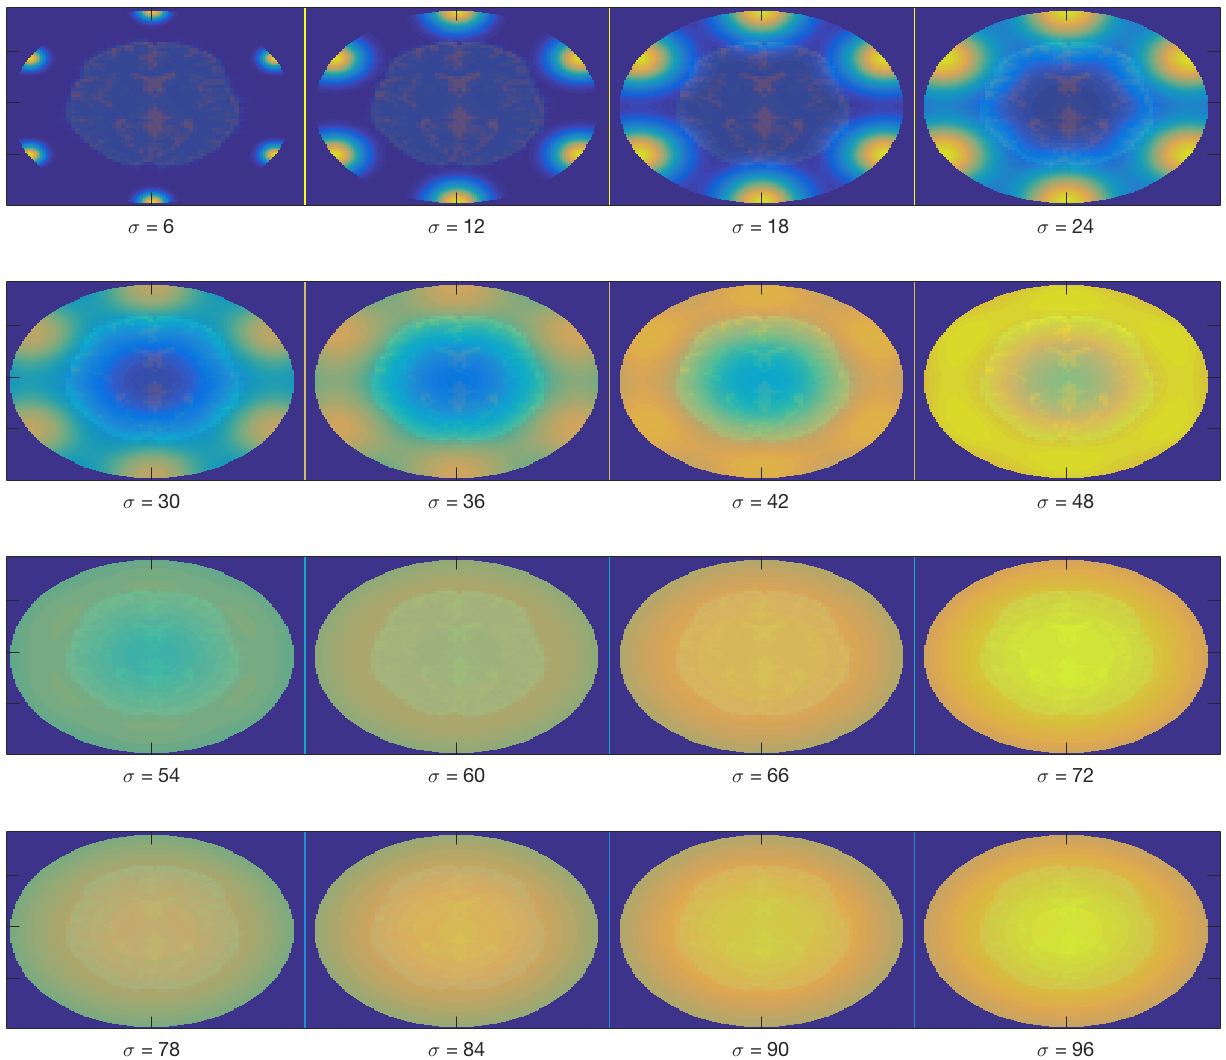
\includegraphics[width=.8\textwidth,keepaspectratio]{6coilsdifsigmas}
    \caption{Coil sensitivity maps of the 6-channel arrangement}
\end{figure}

\begin{figure}[H]
    \centering
    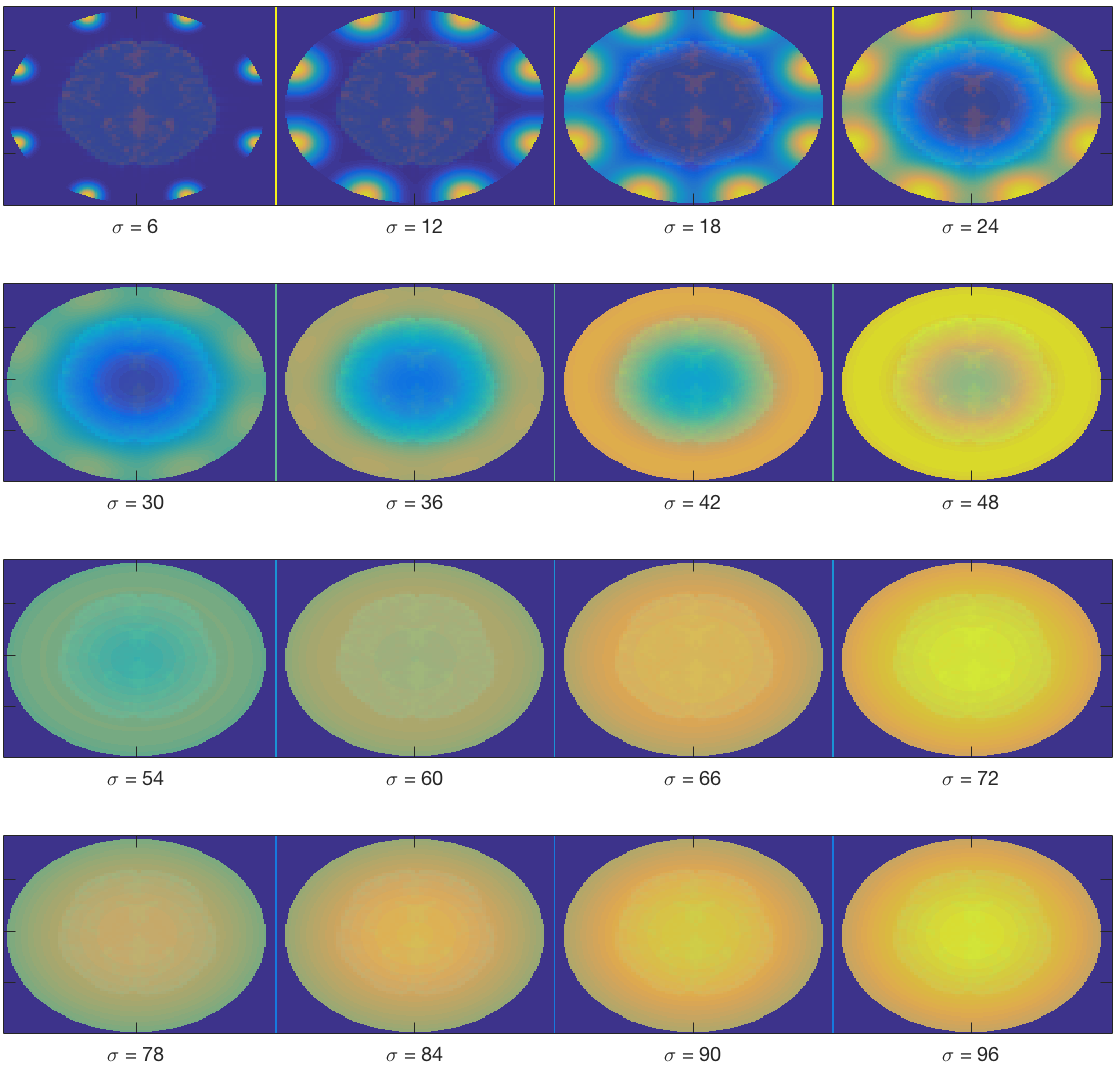
\includegraphics[width=.8\textwidth,keepaspectratio]{8coilsdifsigmas}
    \caption{Coil sensitivity maps of the 8-channel arrangement}
\end{figure}

\begin{figure}[H]
    \centering
    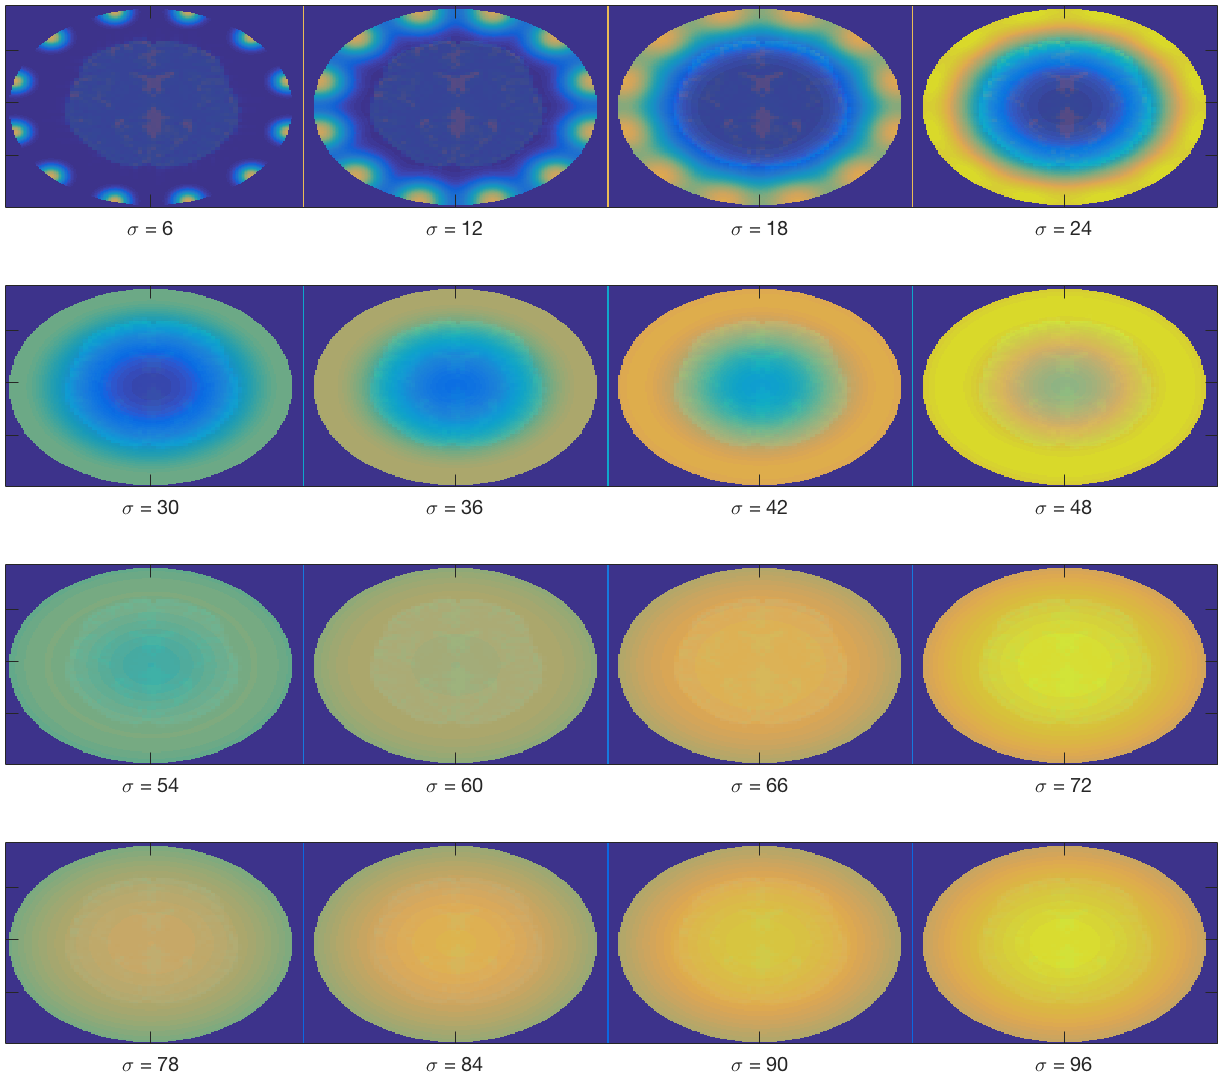
\includegraphics[width=.8\textwidth,keepaspectratio]{12coilsdifsigmas}
    \caption{Coil sensitivity maps of the 12-channel arrangement}
\end{figure}

\begin{figure}[H]
    \centering
    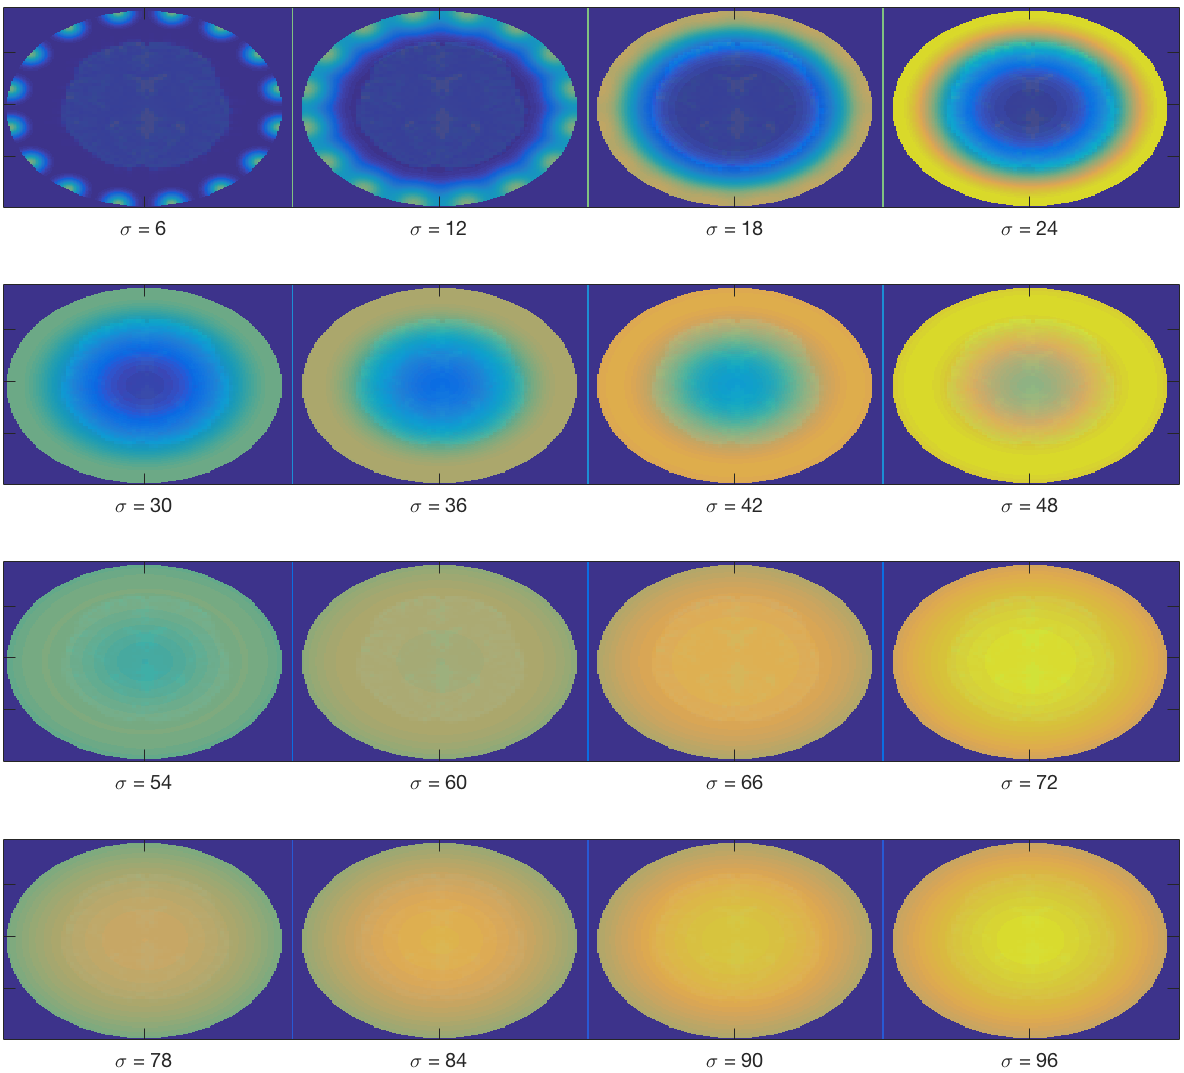
\includegraphics[width=.8\textwidth,keepaspectratio]{16coilsdifsigmas}
    \caption{Coil sensitivity maps of the 16-channel arrangement}
\end{figure}

%%%%%%%%%%%%%%%%%%%%%%%%%%%%%%%%%%%%%%%%%%%%%%%%%%%%%%%%%%%%%%%
%% APPENDIX 2
% \chapter{"g-factor" maps for different acceleration factors}
% \label{appendixlabel2}

% %% R = 1
% \begin{figure}[H]
%     \centering
%     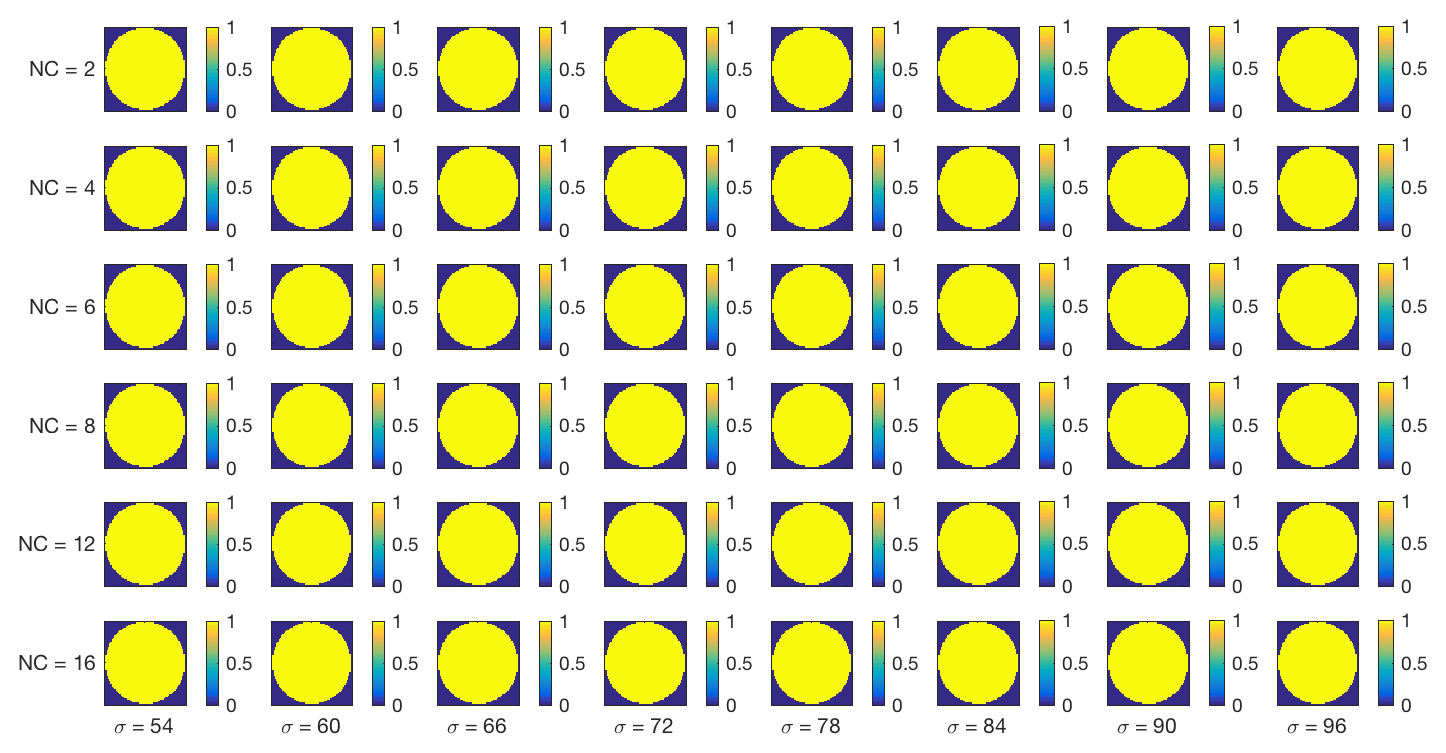
\includegraphics[angle=90,width=.6\textwidth,keepaspectratio]{R1gfactsgm916_new}
%     \caption{g-factor maps for acceleration factor $R = 1$, for increasing numbers of coils on the y-axis and with varying standard deviations of their associated sensitivity profiles on the x-axis}
% \end{figure}

% \begin{figure}[H]
%     \centering
%     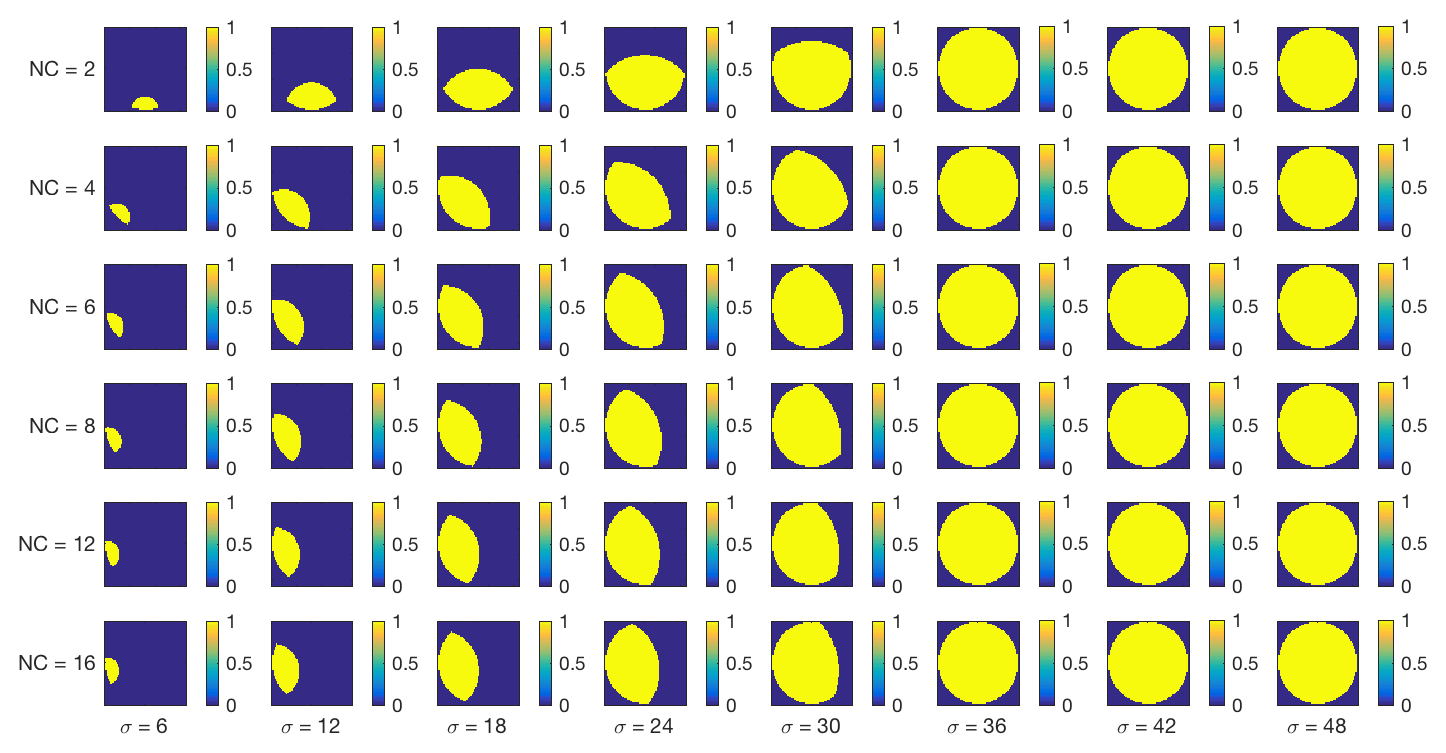
\includegraphics[angle=90,width=.6\textwidth,keepaspectratio]{R1gfactsgm18_new}
%     \caption{g-factor maps for acceleration factor $R = 1$, for increasing numbers of coils on the y-axis and with varying standard deviations of their associated sensitivity profiles on the x-axis}
% \end{figure}

% %% R = 2
% \begin{figure}[H]
%     \centering
%     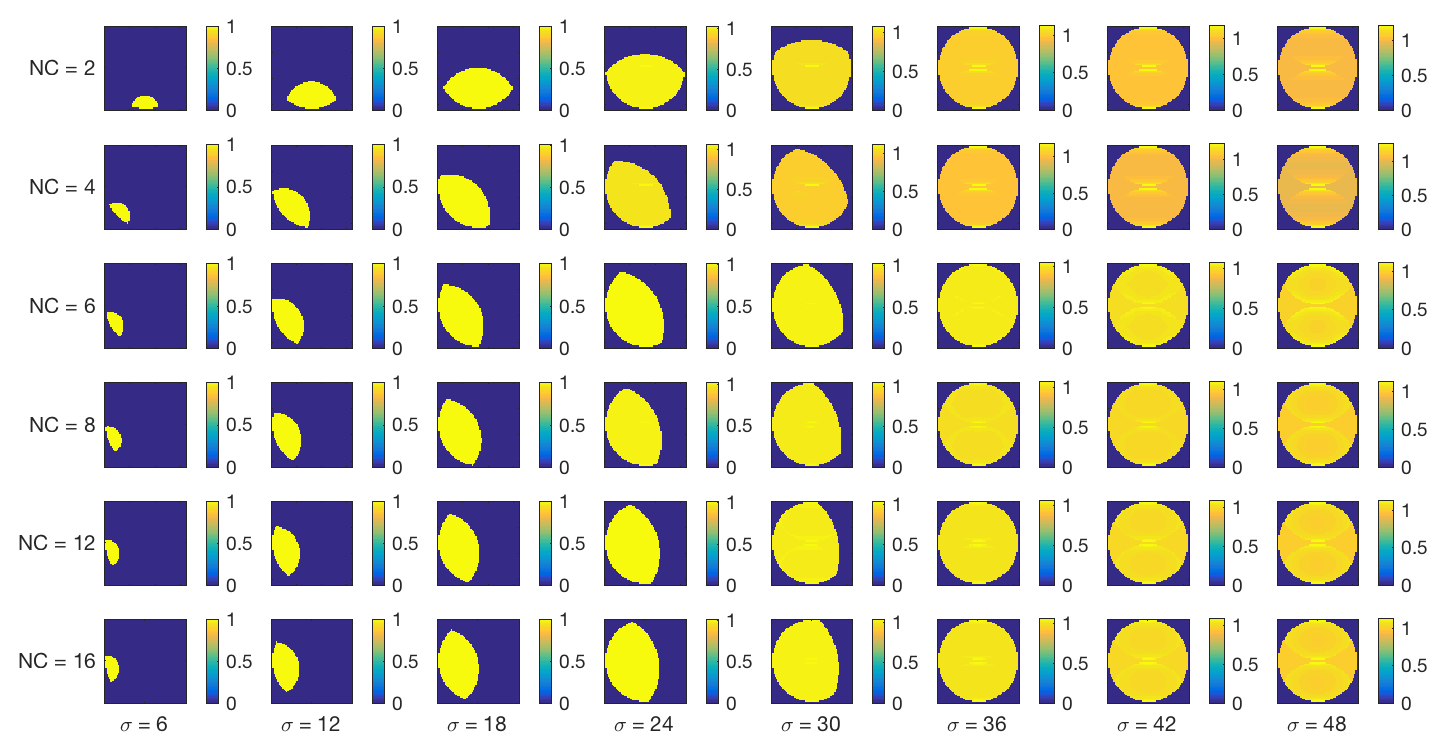
\includegraphics[angle=90,width=.6\textwidth,keepaspectratio]{R2gfactsgm18_new}
%     \caption{g-factor maps for acceleration factor $R = 2$, for increasing numbers of coils on the y-axis and with varying standard deviations of their associated sensitivity profiles on the x-axis}
% \end{figure}

% \begin{figure}[H]
%     \centering
%     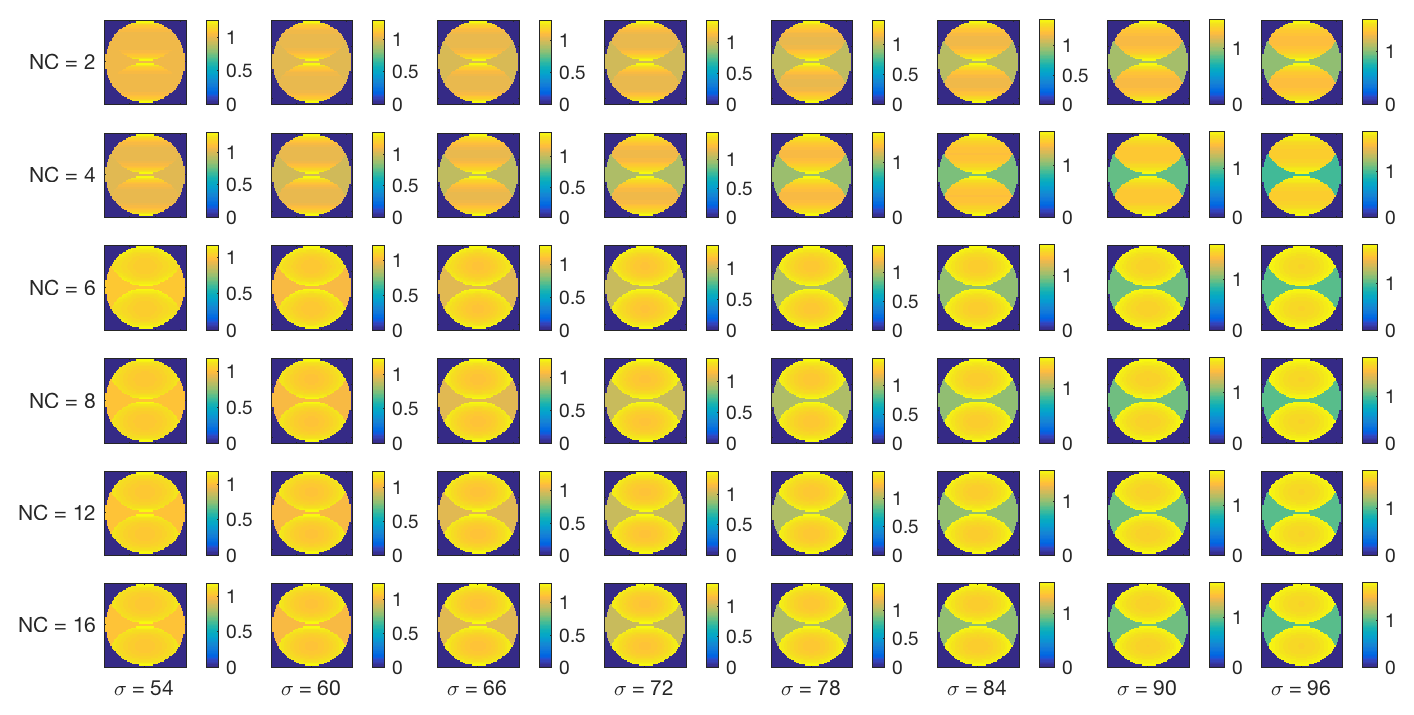
\includegraphics[angle=90,width=.6\textwidth,keepaspectratio]{R2gfactsgm916_new}
%     \caption{g-factor maps for acceleration factor $R = 2$, for increasing numbers of coils on the y-axis and with varying standard deviations of their associated sensitivity profiles on the x-axis}
% \end{figure}

% %% R = 3
% \begin{figure}[H]
%     \centering
%     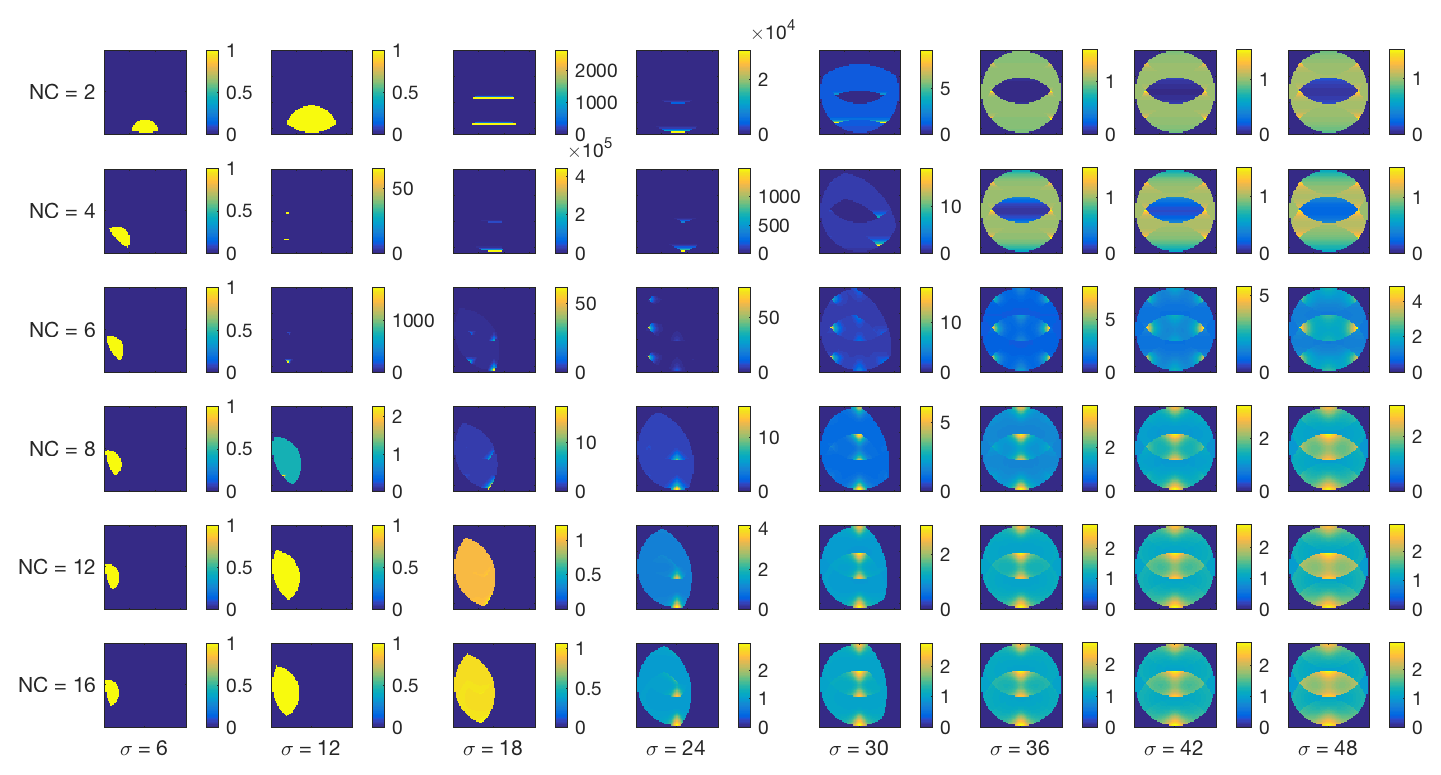
\includegraphics[angle=90,width=.6\textwidth,keepaspectratio]{R3gfactsgm18_new}
%     \caption{g-factor maps for acceleration factor $R = 3$, for increasing numbers of coils on the y-axis and with varying standard deviations of their associated sensitivity profiles on the x-axis}
% \end{figure}

% \begin{figure}[H]
%     \centering
%     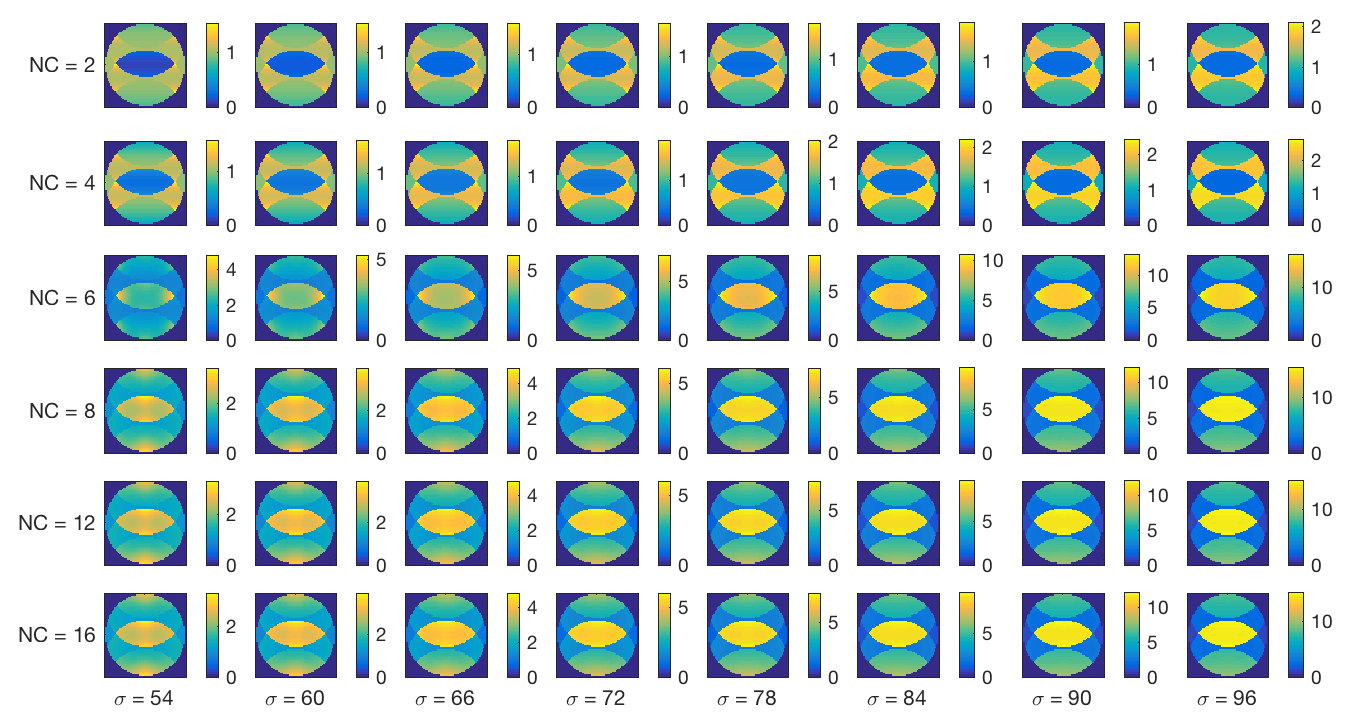
\includegraphics[angle=90,width=.6\textwidth,keepaspectratio]{R3gfactsgm916_new}
%     \caption{g-factor maps for acceleration factor $R = 3$, for increasing numbers of coils on the y-axis and with varying standard deviations of their associated sensitivity profiles on the x-axis}
% \end{figure}

% %% R = 4
% \begin{figure}[H]
%     \centering
%     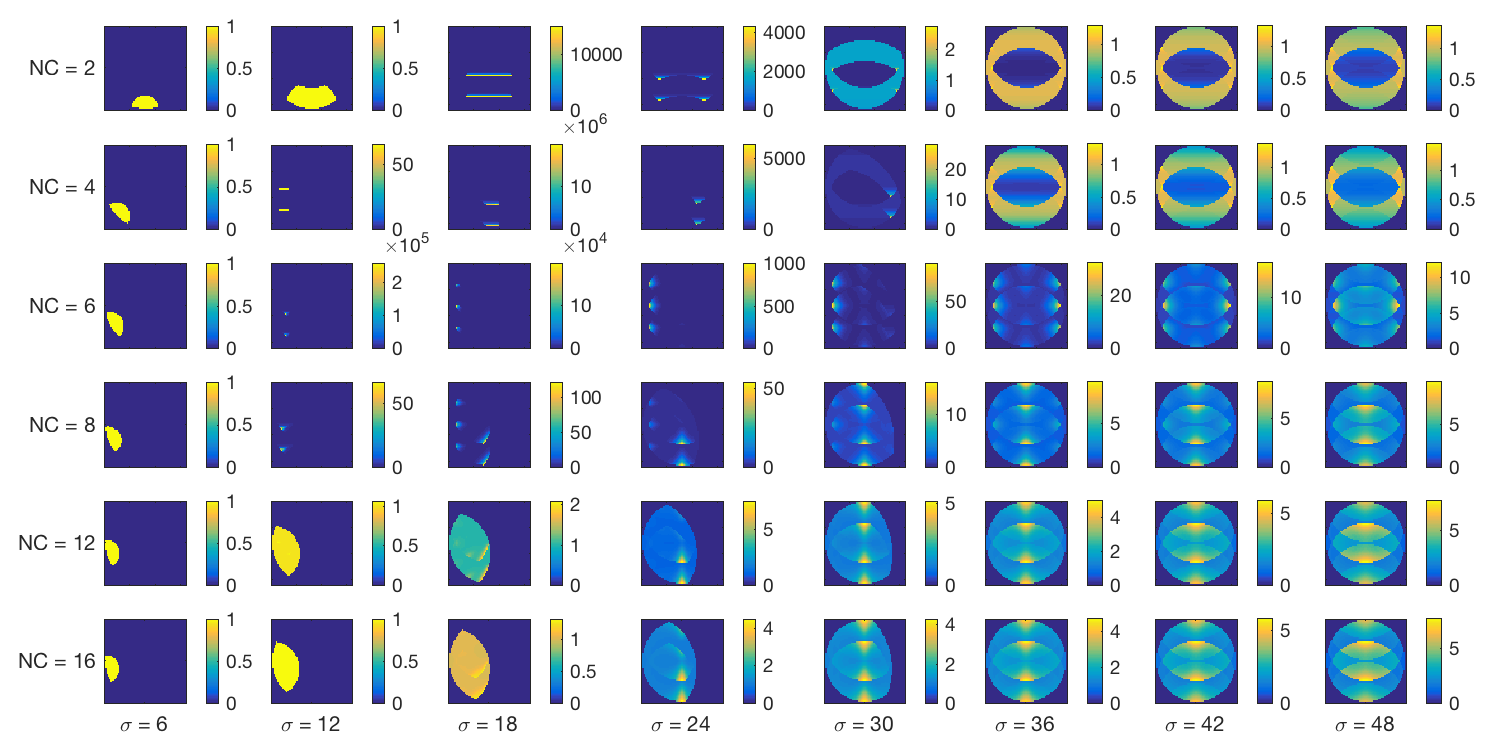
\includegraphics[angle=90,width=.6\textwidth,keepaspectratio]{R4gfactsgm18_new}
%     \caption{g-factor maps for acceleration factor $R = 4$, for increasing numbers of coils on the y-axis and with varying standard deviations of their associated sensitivity profiles on the x-axis}
% \end{figure}

% \begin{figure}[H]
%     \centering
%     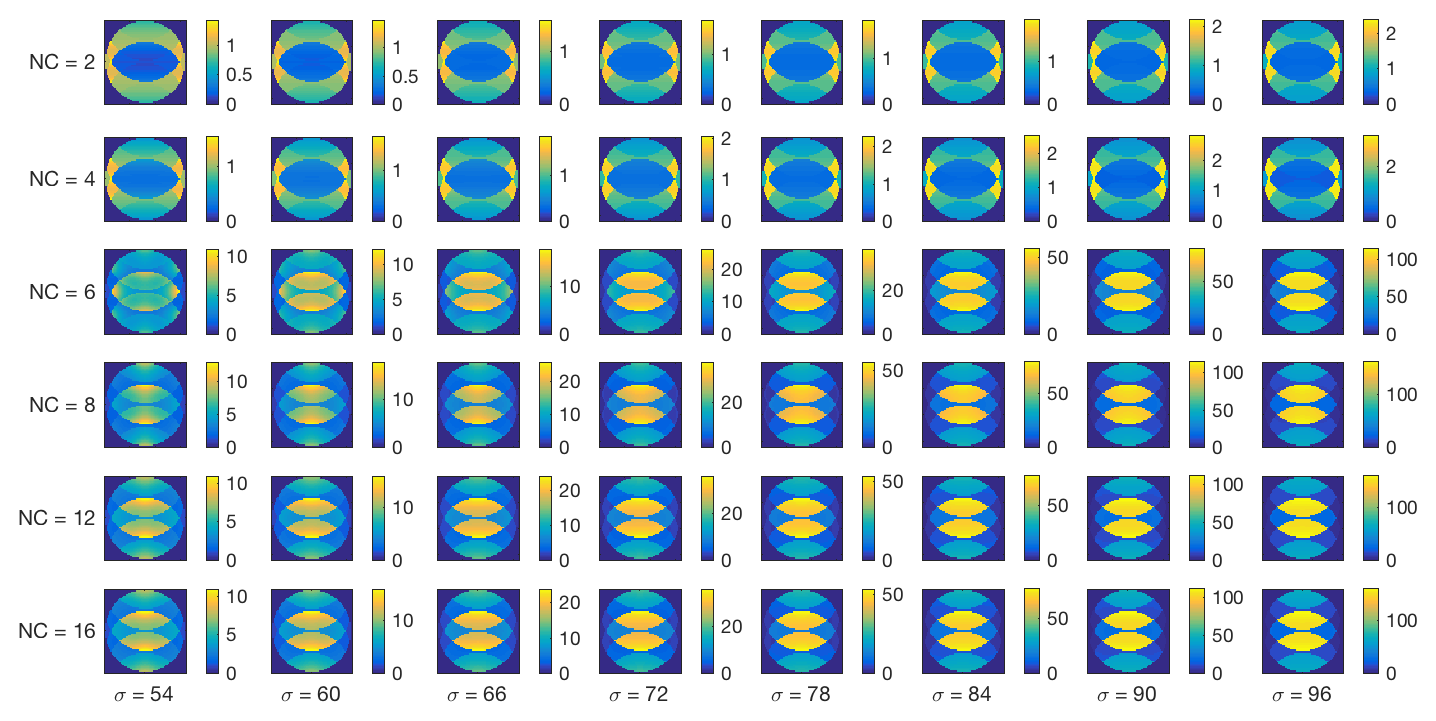
\includegraphics[angle=90,width=.6\textwidth,keepaspectratio]{R4gfactsgm916_new}
%     \caption{g-factor maps for acceleration factor $R = 4$, for increasing numbers of coils on the y-axis and with varying standard deviations of their associated sensitivity profiles on the x-axis}
% \end{figure}


% \chapter{Colophon}
% \label{appendixlabel3}
% \textit{This is a description of the tools you used to make your thesis. It helps people make future documents, reminds you, and looks good.}

% \textit{(example)} This document was set in the Times Roman typeface using \LaTeX\ and Bib\TeX , composed with a text editor. 
 % description of document, e.g. type faces, TeX used, TeXmaker, packages and things used for figures. Like a computational details section.
% e.g. http://tex.stackexchange.com/questions/63468/what-is-best-way-to-mention-that-a-document-has-been-typeset-with-tex#63503

% Side note:
%http://tex.stackexchange.com/questions/1319/showcase-of-beautiful-typography-done-in-tex-friends